\hypertarget{Node_8c}{
\section{Node.c File Reference}
\label{Node_8c}\index{Node.c@{Node.c}}
}
{\tt \#include \char`\"{}party.h\char`\"{}}\par


Include dependency graph for Node.c:\nopagebreak
\begin{figure}[H]
\begin{center}
\leavevmode
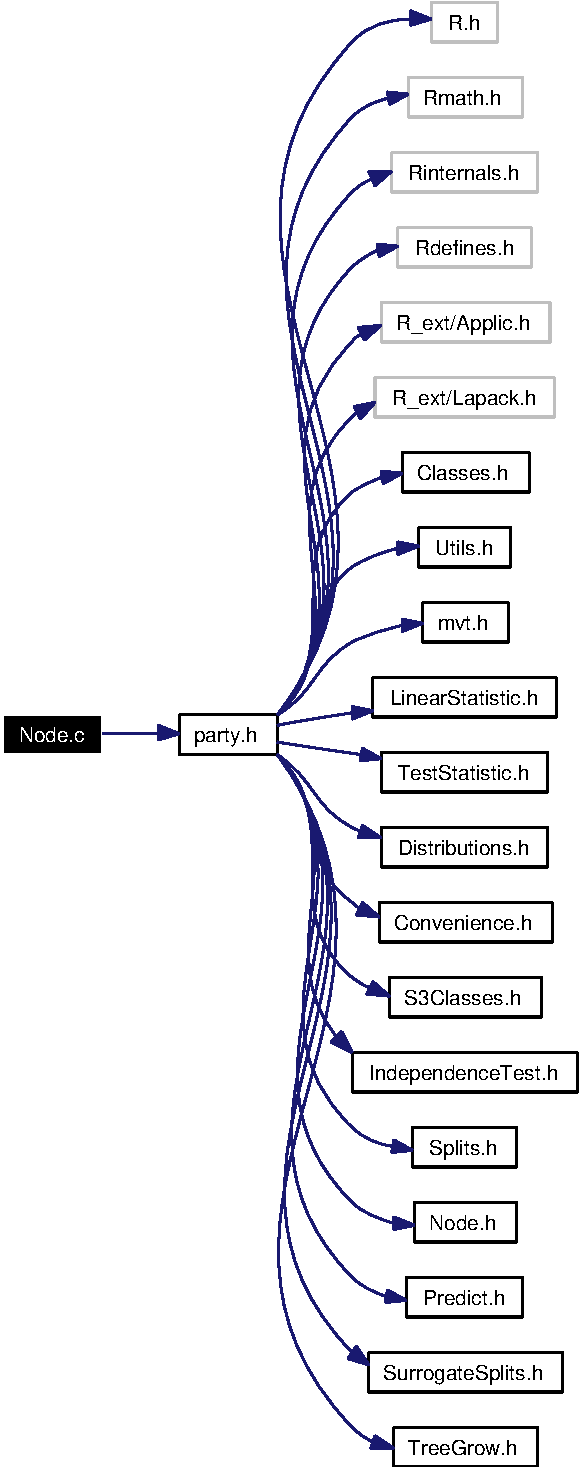
\includegraphics[width=420pt]{Node_8c__incl}
\end{center}
\end{figure}
\subsection*{Functions}
\begin{CompactItemize}
\item 
void \hyperlink{Node_8c_ccc1b172efcfd43dc460efee333b6abf}{C\_\-prediction} (const double $\ast$y, int n, int q, const double $\ast$weights, const double sweights, double $\ast$ans)
\item 
void \hyperlink{Node_8c_0ed8b15b2c14ec9f1f1585d6288a38e2}{C\_\-Node} (SEXP node, SEXP learnsample, SEXP weights, SEXP fitmem, SEXP controls, int TERMINAL)
\item 
SEXP \hyperlink{Node_8c_878214ca472c99cf036a426eb7cffb59}{R\_\-Node} (SEXP learnsample, SEXP weights, SEXP fitmem, SEXP controls)
\end{CompactItemize}


\subsection{Detailed Description}
Node computations

\begin{Desc}
\item[Author:]\begin{Desc}
\item[Author]\end{Desc}
\end{Desc}
\begin{Desc}
\item[Date:]\begin{Desc}
\item[Date]\end{Desc}
\end{Desc}


Definition in file \hyperlink{Node_8c-source}{Node.c}.

\subsection{Function Documentation}
\hypertarget{Node_8c_0ed8b15b2c14ec9f1f1585d6288a38e2}{
\index{Node.c@{Node.c}!C_Node@{C\_\-Node}}
\index{C_Node@{C\_\-Node}!Node.c@{Node.c}}
\subsubsection{\setlength{\rightskip}{0pt plus 5cm}void C\_\-Node (SEXP {\em node}, SEXP {\em learnsample}, SEXP {\em weights}, SEXP {\em fitmem}, SEXP {\em controls}, int {\em TERMINAL})}}
\label{Node_8c_0ed8b15b2c14ec9f1f1585d6288a38e2}


The main function for all node computations \begin{Desc}
\item[Parameters:]
\begin{description}
\item[{\em node}]an initialized node (an S3 object!) \item[{\em learnsample}]an object of class `LearningSample' \item[{\em weights}]case weights \item[{\em fitmem}]an object of class `TreeFitMemory' \item[{\em controls}]an object of class `TreeControl' \item[{\em TERMINAL}]logical indicating if this node will be a terminal node \end{description}
\end{Desc}


Definition at line 48 of file Node.c.

Referenced by C\_\-TreeGrow(), and R\_\-Node().\hypertarget{Node_8c_ccc1b172efcfd43dc460efee333b6abf}{
\index{Node.c@{Node.c}!C_prediction@{C\_\-prediction}}
\index{C_prediction@{C\_\-prediction}!Node.c@{Node.c}}
\subsubsection{\setlength{\rightskip}{0pt plus 5cm}void C\_\-prediction (const double $\ast$ {\em y}, int {\em n}, int {\em q}, const double $\ast$ {\em weights}, const double {\em sweights}, double $\ast$ {\em ans})}}
\label{Node_8c_ccc1b172efcfd43dc460efee333b6abf}


Compute prediction of a node \begin{Desc}
\item[Parameters:]
\begin{description}
\item[{\em y}]the response variable (raw numeric values or dummy encoded factor) \item[{\em n}]number of observations \item[{\em q}]number of columns of y \item[{\em weights}]case weights \item[{\em sweights}]sum of case weights \item[{\em ans}]return value; the q-dimensional predictions \end{description}
\end{Desc}


Definition at line 22 of file Node.c.

Referenced by C\_\-Node().\hypertarget{Node_8c_878214ca472c99cf036a426eb7cffb59}{
\index{Node.c@{Node.c}!R_Node@{R\_\-Node}}
\index{R_Node@{R\_\-Node}!Node.c@{Node.c}}
\subsubsection{\setlength{\rightskip}{0pt plus 5cm}SEXP R\_\-Node (SEXP {\em learnsample}, SEXP {\em weights}, SEXP {\em fitmem}, SEXP {\em controls})}}
\label{Node_8c_878214ca472c99cf036a426eb7cffb59}


R-interface to C\_\-Node \begin{Desc}
\item[Parameters:]
\begin{description}
\item[{\em learnsample}]an object of class `LearningSample' \item[{\em weights}]case weights \item[{\em fitmem}]an object of class `TreeFitMemory' \item[{\em controls}]an object of class `TreeControl' \end{description}
\end{Desc}


Definition at line 227 of file Node.c.

References C\_\-init\_\-node(), C\_\-Node(), get\_\-maxsurrogate(), get\_\-ninputs(), get\_\-nobs(), get\_\-predict\_\-trafo(), get\_\-splitctrl(), ncol(), NODE\_\-LENGTH, and PL2\_\-responsesSym.

Here is the call graph for this function:\nopagebreak
\begin{figure}[H]
\begin{center}
\leavevmode
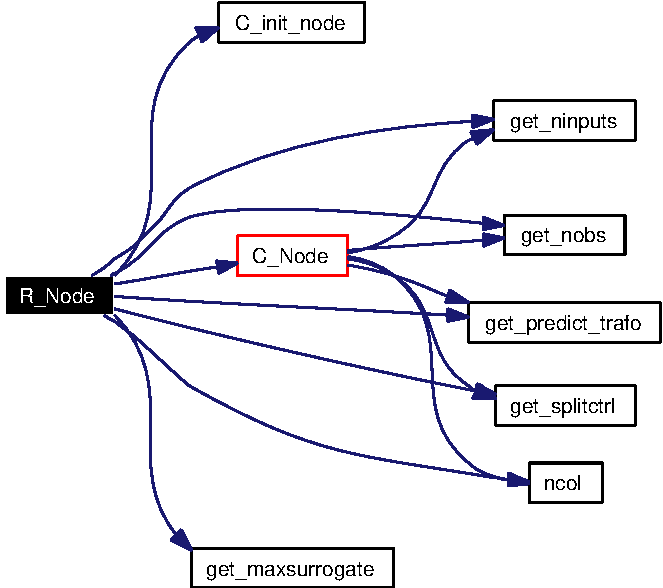
\includegraphics[width=120pt]{Node_8c_878214ca472c99cf036a426eb7cffb59_cgraph}
\end{center}
\end{figure}
